\documentclass[10pt,twoside]{article}
\usepackage[a4paper,margin=2.2cm]{geometry}
\usepackage{amsmath,amssymb}
\usepackage{graphicx}
\usepackage{booktabs}
\usepackage[font=small,labelfont=bf,labelsep=period]{caption}
\usepackage[numbers,sort&compress]{natbib}
\usepackage{microtype}
\usepackage{xcolor}
\usepackage[colorlinks=true,linkcolor=blue!50!black,citecolor=blue!50!black,urlcolor=blue!50!black]{hyperref}
\usepackage{float}
\setlength{\parskip}{0pt}
\renewcommand{\figurename}{FIG.}
\renewcommand{\tablename}{TABLE}
\newcommand{\hb}{\bar h}

\title{\textbf{One dimer manifold, many crystals:\\ height plateaus, wall crystals and design rules in Cairo--Shakti artificial spin ice}}
\author{Changyeon Won\\[2pt]
\small Department of Physics, Kyung Hee University, Seoul 02447, Republic of Korea\\
\small \texttt{cywon@khu.ac.kr}}
\date{}

\begin{document}
\maketitle

\begin{abstract}
\noindent
Vertex-frustrated artificial spin ices such as the Shakti lattice owe their extensive degeneracy to a mapping onto dimer coverings, but what selects an ordered state out of that degeneracy, and why experiments rarely see it, has remained unclear. We study a one-parameter family of pentagonal lattices, Cairo$(d)$, that interpolates continuously from square ice through the equilateral Cairo lattice to the Shakti lattice. Three results emerge. First, the low-energy manifold is topological: for every $d$ in a wide window it is exactly the set of dimer coverings of the square lattice, with exactly half of all pentagons carrying a closed vortex. Second, the long-range dipolar interaction acts on this manifold as a locking potential for the dimer height field. All selected states are flat height plateaus---a bond-ordered basketweave crystal (A), a sublattice-ordered basketweave crystal (C), a columnar crystal---or dense crystals of sharp, nearly non-interacting walls between plateaus: the wall crystal W in the basketweave family and the ladder crystal L3$'$ in the columnar family. Whether walls proliferate is set by the sign of a single wall tension, which is fixed by distant island pairs only and therefore depends on island shape through one number, the moment ratio $\mu=m_{\rm long}/m_{\rm short}$. W is stable for $\mu_c(d)<\mu<\mu_A(d)$, with $\mu_c\simeq1.2$--$1.8$. Third, small symmetry-breaking deformations---anisotropy, twist and axial strain---couple linearly to the order parameters through an exact vertex-level identity, so that sub-degree twists or nanometre displacements select A, C, W or the columnar crystal. Applied to the islands of the dipolar Cairo lattice of Saccone \emph{et al.}, the theory identifies the ground state as A, with an ordering temperature of 320--560~K that lies well below the effective freezing temperature inferred from the measured vertex populations, which explains the absence of long-range order. In finite Aztec-diamond regions the boundary pins the plateau height to $\pm(n+1)$ mod 4, so that the selected crystal alternates with the size parity. These results turn the Cairo--Shakti family into a set of design rules for ordered states in vertex-frustrated magnets.
\end{abstract}

\section{Introduction}

Artificial spin ices---lithographic arrays of single-domain nanomagnets whose Ising moments interact through dipolar fields---make frustration directly visible~\cite{Wang2006,Nisoli2013,Skjaervo2020}. A central lesson of the field is that geometry, not only the strength of interactions, decides what a frustrated magnet does. In square ice the vertex energies select a unique ground state; in kagome ice they leave an ice manifold that long-range interactions reorganise into charge-ordered and loop-ordered phases~\cite{Moller2009}. Vertex-frustrated lattices go one step further: mixed coordination prevents all vertices from reaching their lowest energy simultaneously, and the resulting degeneracy is topological rather than accidental~\cite{Morrison2013,Chern2013}. The Shakti lattice is the paradigm. Its ground states map onto dimer coverings of the square lattice, it displays an emergent ice rule and screened magnetic charges~\cite{Chern2013,Gilbert2014,Stopfel2018}, and its kinetics carry signatures of classical topological order~\cite{Lao2018}.

The pentagonal Cairo lattice belongs to the same topological class~\cite{Saccone2019,RodriguezGallo2023a}. Thermally annealed Cairo arrays show an emergent ice rule but only short-range correlations~\cite{Saccone2019}; exhaustive enumeration of small dipolar Cairo clusters finds ground states that differ from the configurations with the maximal number of closed pentagons~\cite{Makarova2021}; and colloidal Cairo and Shakti--Cairo ices reveal how geometry controls the transfer of topological charge~\cite{RodriguezGallo2023a,RodriguezGallo2023b}. Pentagonal motifs also appear in artificial quasicrystals, whose vortex textures motivated the present work~\cite{Farmer2016,Shi2018}. Three questions remain open. What, precisely, is the degenerate manifold of a Cairo-type magnet, and how does it depend on the lattice geometry? Which ordered state do long-range interactions select, and why? And why do experiments see disorder?

Here we answer these questions for a continuous family of lattices, Cairo$(d)$ [Fig.~\ref{fig:family}], which contains the equilateral Cairo lattice and the Shakti lattice as special points. Our main findings are the following.
(i) The low-energy manifold is exactly the set of square-lattice dimer coverings for all $0.07\lesssim d\lesssim0.48$; the number of states and the fraction of closed pentagons (exactly one half) follow from the dimer model.
(ii) All selected states are organised by the dimer height field. Basketweave crystals sit on integer height plateaus, columnar crystals on half-integer plateaus; the equilibrium phases are either flat plateaus or dense crystals of sharp walls between them, namely W for basketweave and the ladder crystal L3$'$ for columnar order.
(iii) An exact vertex-level identity makes small symmetry-breaking deformations act as strong, linear fields on the order parameters, with a selection rule fixed by symmetry.
(iv) The wall tension that decides between C and W comes only from distant island pairs, so island shape enters through the moment ratio $\mu$ alone; this yields an analytic phase diagram in the $(d,\mu)$ plane that realistic island calculations confirm.
(v) For the measured Cairo arrays the ground state is A, but the arrays freeze far above its ordering temperature.
(vi) In finite regions the boundary pins the height plateau, so that the selected crystal alternates with the parity of the system size.

\begin{figure}[t]
\centering
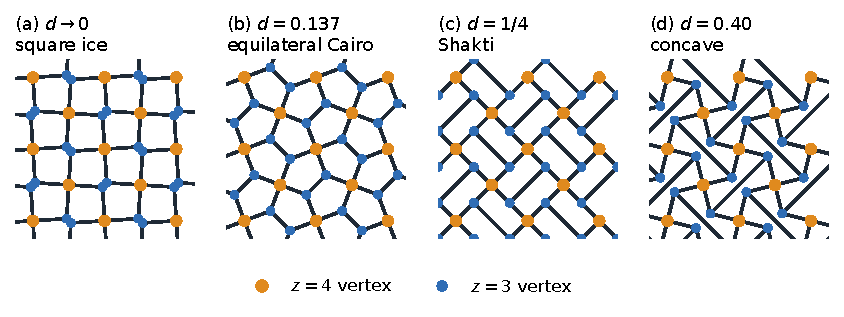
\includegraphics[width=\textwidth]{figs/fig1_family.pdf}
\caption{The Cairo$(d)$ family. Islands sit on the edges; $z=4$ vertices (orange) are fixed and the two $z=3$ vertices of each partner pair (blue) are separated by $d$. (a) $d\to0$ approaches square ice; (b) $d=(\sqrt7-1)/12\simeq0.137$ is the equilateral Cairo lattice; (c) $d=1/4$ is the Shakti lattice, in which the partner bond becomes a long island; (d) $d>1/4$ gives concave pentagons.}
\label{fig:family}
\end{figure}

\section{Model}

The lattice has $p4g$ symmetry with $z=4$ vertices at $(0,0)$ and $(\tfrac12,\tfrac12)$ and two pairs of $z=3$ vertices at $(\tfrac12\pm d,\pm d)$ and $(\mp d,\tfrac12\pm d)$, giving ten islands, six vertices and four pentagons per unit cell. Each island carries an Ising moment along its edge. The energy is the full dipolar energy
\begin{equation}
E=\frac12\sum_{i\neq j}J_{ij}\,s_is_j,\qquad s_i=\pm1,
\label{eq:energy}
\end{equation}
summed over periodic images. We use two island models. In the \emph{ideal} model each island is a uniformly magnetised needle filling its edge, discretised into point sub-dipoles; the long partner island of the Shakti lattice then carries twice the moment of a short island. In the \emph{realistic} model each island is a stadium of width 100~nm and thickness 3~nm with $M_s=790$~kA/m, separated from the vertices by fixed gaps (86~nm for islands touching $z=4$ vertices, 22~nm for partner islands), which reproduces the islands of Ref.~\cite{Saccone2019} at $d=0.105$. Couplings between islands sharing a vertex define the vertex energies; all other pairs are summed with an island-level cutoff of $\geq24a$, where $a$ is the length of a $z3$--$z4$ edge (Appendix~\ref{app:methods}). Energies of different crystals are always compared on a common torus, since self-image terms add a state-independent but size-dependent constant.

\section{Topology: an exact dimer manifold}

For each $z=3$ vertex the three possible two-in--one-out configurations split into a lower doublet (``happy'') and an upper quartet (``unhappy''). Vertex frustration forces exactly half of all $z=3$ vertices to be unhappy when all $z=4$ vertices are in their lowest (type-I) state. Every unhappy vertex has exactly one $z3$--$z4$ island whose reversal would heal it; the two pentagons sharing that island form a domino. Because pentagons connected through $z3$--$z4$ edges form a square lattice, the low-energy configurations are in one-to-one correspondence with dimer coverings of that square lattice [Fig.~\ref{fig:ACW}(d)--(f)]. We verified the bijection by exhaustive enumeration on periodic cells up to $4\times3$; the number of states is
\begin{equation}
W(n_x,n_y)=2\,Z_{\rm dimer}(2n_x\times2n_y),
\end{equation}
with the winding sector fixed by the parities of $n_x,n_y$ (39\,952 states on the $4\times2$ cell). The manifold is identical as a set of spin configurations for all $0.07\lesssim d\lesssim0.48$ in the ideal model, so that the equilateral Cairo and the Shakti lattices share one and the same manifold. Two simple rules follow. Every domino joins one closed pentagon (circulation $|\chi|=1$) and one open pentagon of the same circulation sense, so that \emph{exactly one half of all pentagons are closed} in every ground state; configurations with more closed pentagons necessarily contain extra unhappy vertices. This explains the observation of Ref.~\cite{Makarova2021} that ground states do not maximise the number of closed pentagons. The residual entropy is that of square-lattice dimers, $2G/\pi\simeq0.583$ per domino, with $G$ Catalan's constant~\cite{Kasteleyn1961}.

\begin{figure}[t]
\centering
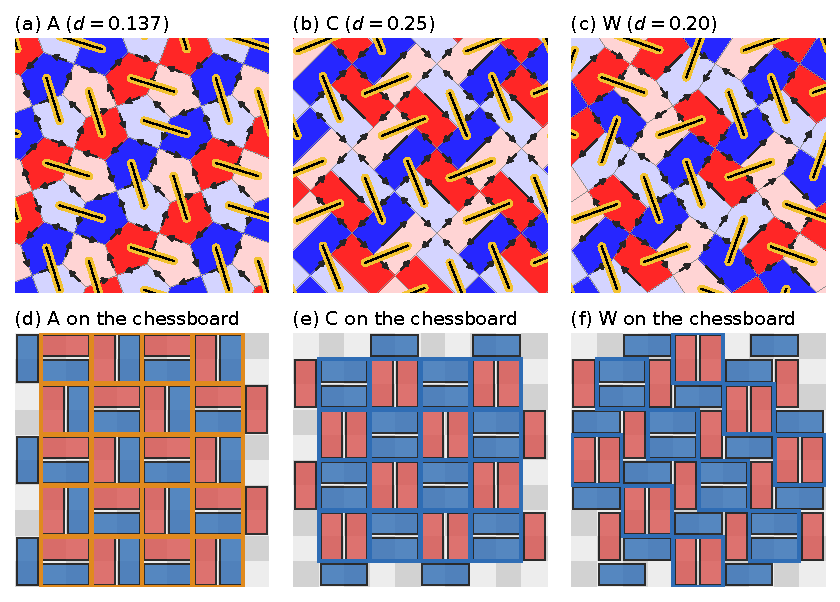
\includegraphics[width=\textwidth]{figs/fig2_ACW.pdf}
\caption{The selected crystals in real space (top) and as domino tilings of the pentagon chessboard (bottom). Colours give the pentagon circulation (red clockwise, blue counter-clockwise); yellow bars are dominoes. Outlined squares mark flippable $2\times2$ blocks, coloured by the parity of their origin (blue: even, centred on $z=4$ vertices; orange: odd, centred on partner bonds). (a,d) A at the equilateral Cairo point: basketweave with blocks on partner bonds. (b,e) C at the Shakti point: basketweave with blocks on $z=4$ vertices. (c,f) The wall crystal W: C and C$'$ domains separated by dense walls.}
\label{fig:ACW}
\end{figure}

\section{Selection: height plateaus}

\subsection{Basketweave crystals and the height clock}

Within the manifold all vertex energies are equal, so selection is done entirely by islands that do not share a vertex. Exact enumeration of the $4\times2$ manifold with converged dipolar sums finds two crystals [Fig.~\ref{fig:ACW}]: A on the Cairo side and C on the Shakti side. On the chessboard both are the \emph{same} basketweave tiling---$2\times2$ blocks of two parallel dominoes alternating between horizontal and vertical---and they differ only in which class of plaquettes the blocks occupy. The plaquettes of the chessboard are of four kinds, centred on the two $z=4$ sublattices or on the two partner-bond orientations. Blocks centred on $z=4$ vertices give C; blocks centred on partner bonds give A.

The Thurston height function of the dimer covering~\cite{Thurston1990,Henley2010} makes this precise [Fig.~\ref{fig:height}]. The four placements of the basketweave are flat states at the four heights $\hb\equiv0,1,2,3$ (mod 4): C occupies the even plateaus and A the odd ones. The order parameters are harmonics of the plateau height,
\begin{equation}
\psi_C=\cos\frac{\pi\hb}{2},\qquad\psi_A=\sin\frac{\pi\hb}{2},\qquad\Phi=\cos\pi\hb=\psi_C^2-\psi_A^2,
\end{equation}
where $\Phi$ distinguishes A from C without breaking any lattice symmetry. A coarse-grained free energy
\begin{equation}
F[\hb]=\int d^2x\left[\frac K2|\nabla\hb|^2+V(\hb)\right]+\frac12\iint(\hat z\times\nabla\hb)\cdot\mathsf D(\mathbf x-\mathbf x')\cdot(\hat z\times\nabla\hb'),
\qquad V=-u\cos2\pi\hb-\delta\cos\pi\hb,
\label{eq:F}
\end{equation}
summarises the selection: $\delta$ chooses between even (C) and odd (A) plateaus and changes sign at the A$|$C boundary $d_c$; the sign of $u$ chooses between integer heights (basketweave) and half-integer heights (columnar crystals)~\cite{Fradkin2004,Alet2005}; the last term is the long-range dipolar coupling of the coarse-grained magnetisation $\hat z\times\nabla\hb$.

\begin{figure}[t]
\centering
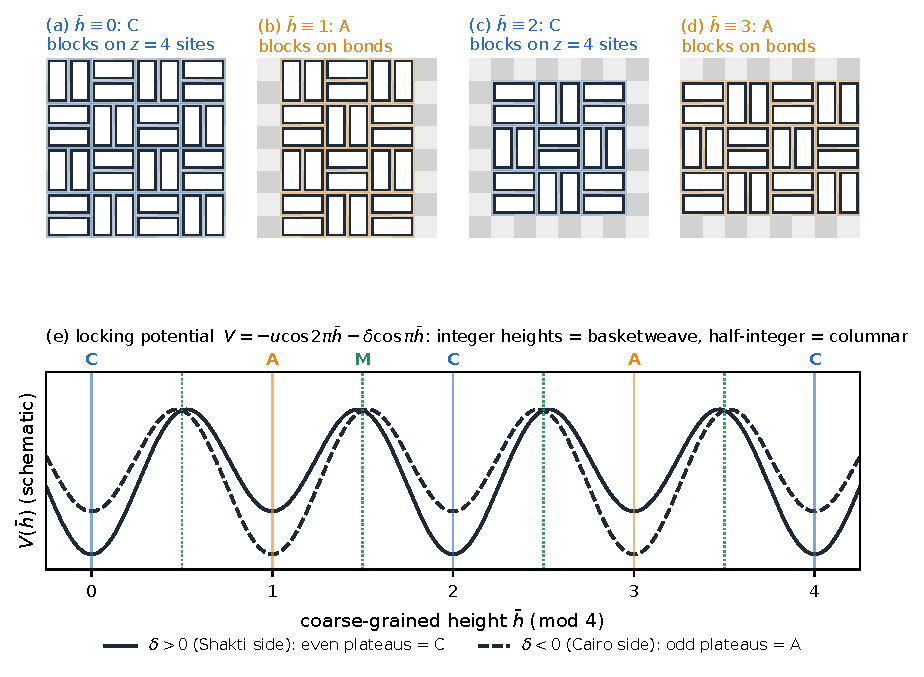
\includegraphics[width=\textwidth]{figs/fig3_height.pdf}
\caption{Height plateaus. (a)--(d) The four placements of the basketweave tiling sit on the four plateau heights $\hb\equiv0,1,2,3$ (mod 4); even plateaus are C, odd plateaus are A. (e) Schematic locking potential: the sign of $\delta$ selects even or odd plateaus, while columnar states (M) sit at half-integer heights.}
\label{fig:height}
\end{figure}

\subsection{Between A and C: the ladder crystal}

Comparing all candidates on a common torus reveals that A and C do not meet directly [Fig.~\ref{fig:ladder}(c)]. In a narrow window $0.1495\lesssim d\lesssim0.157$ around $d_c\simeq0.153$ the ground state of the ideal model is a ladder crystal, L3$'$: single layers of columnar dominoes separated by single rows of horizontal dominoes whose phase alternates regularly [Fig.~\ref{fig:ladder}(b),(e)]. In the uniform columnar crystal M [Fig.~\ref{fig:ladder}(a),(d)] all rows of parallel dominoes are stacked into ladders, and the local mean height is $\hb=\tfrac12$ everywhere. In L3$'$ the local block plateaus alternate between $\{2,3\}$ and $\{0,1\}$, so that the local mean height jumps between $\tfrac12$ and $\tfrac52$ at every horizontal row [Fig.~\ref{fig:ladder}(f)]: L3$'$ is a dense crystal of walls between two columnar variants. A ladder crystal with irregular phases had first been found by parallel tempering on $12\times12$ tori; the regular-phase L3$'$ is lower by $5\times10^{-4}$ (in units of $D/a^3$ per island) at every $d$, which illustrates how glassy the dynamics is in this window. At finite temperature, at $d=0.145$, finite-size scaling up to 5760 islands shows that A melts through a transition with a finite latent heat ($8.3\times10^{-3}$ per island) and a size-converged transition temperature, but with a free-energy barrier that stops growing beyond $n\approx16$ and a specific-heat peak scaling as $N^{0.89}$; the high-energy branch is not the C crystal but a state with strongly fluctuating A and C correlations. The transition is therefore a weak first-order transition or a pseudo-first-order crossover.

\begin{figure}[t]
\centering
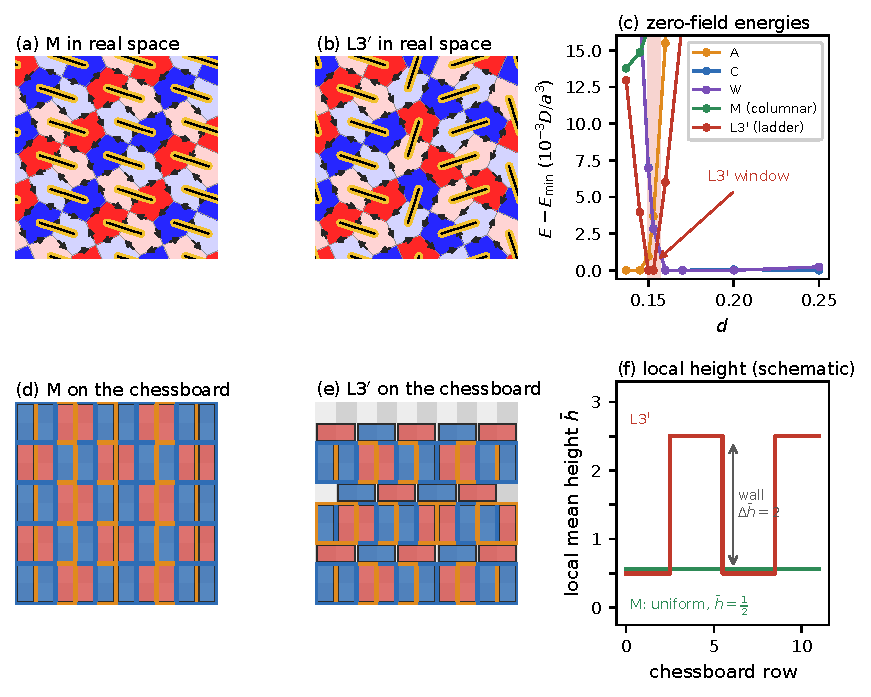
\includegraphics[width=\textwidth]{figs/fig4_ladder.pdf}
\caption{The columnar crystal M and the ladder crystal L3$'$. (a),(b) Real space (pentagon circulation, island moments and dominoes as in Fig.~\ref{fig:ACW}). (c) Zero-field energies of all candidate crystals (ideal islands, common $12\times4$ torus): L3$'$ is the ground state in a narrow window between A and C$\simeq$W. (d),(e) The same states on the chessboard: in M all ladders are stacked; in L3$'$ single columnar layers are separated by horizontal rows. (f) Schematic local mean height across the rows: M is a flat half-integer plateau, L3$'$ a dense crystal of walls with $\Delta\hb=2$.}
\label{fig:ladder}
\end{figure}

\section{Symmetry breaking: an exact vertex-level identity}

Real arrays are never perfectly symmetric. We therefore consider three simple deformations that preserve the topology [Fig.~\ref{fig:defshape}]: diagonal anisotropy $\varepsilon=d_1-d_2$ between the two partner-pair orientations, which breaks the four-fold rotation $R$; a twist $\theta$ of each partner pair about its centre, which keeps $R$ but breaks the diagonal mirror $M$; and axial strain $\eta$, which distinguishes the two lattice axes.

\begin{figure}[t]
\centering
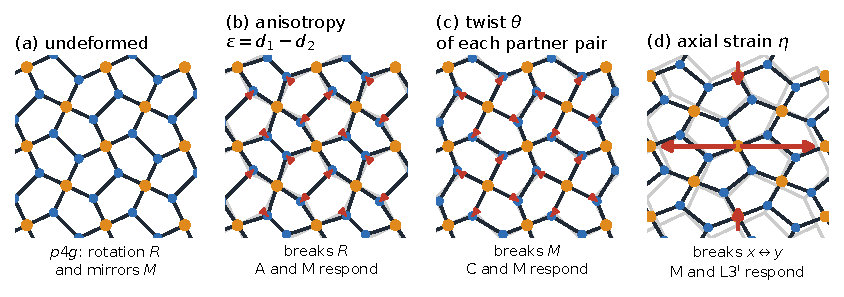
\includegraphics[width=\textwidth]{figs/fig5_deformations.pdf}
\caption{The three topology-preserving deformations, strongly exaggerated (grey: undeformed lattice; red arrows: displacements of the $z=3$ vertices). (b) Anisotropy moves the two partner-pair orientations apart by different amounts and breaks the four-fold rotation $R$. (c) A twist rotates each partner pair about its centre and breaks the mirrors $M$ while keeping $R$. (d) Axial strain stretches one lattice axis and compresses the other. The crystals that respond linearly to each deformation are indicated (see Table~\ref{tab:response}).}
\label{fig:defshape}
\end{figure} The order parameters transform as $\psi_A\colon(R,M)=(-,+)$ and $\psi_C\colon(+,-)$, so $\varepsilon$ couples linearly to $\psi_A$ and $\theta$ to $\psi_C$.

The coupling turns out to be exact and strong. A deformation changes the cost of an unhappy vertex differently for the two choices it distinguishes---which partner set, or which $z=4$ sublattice, the healing domino points to. Since $\psi_A$ and $\psi_C$ count exactly these choices, the vertex energy on the manifold is
\begin{equation}
E_{\rm vertex}=E_0-\lambda_A\,\varepsilon\,\psi_A-\lambda_C\,\theta\,\psi_C,\qquad \lambda_A=\frac{\Delta_{\rm set\,1}-\Delta_{\rm set\,2}}{10\,\varepsilon},
\label{eq:identity}
\end{equation}
where $\Delta_{\rm set}$ is the happy--unhappy splitting of a $z=3$ vertex in each partner set and the factor 10 counts islands per unit cell. Equation~\eqref{eq:identity} holds to $10^{-13}$ over the whole manifold. Because it acts at the vertex level, it is far stronger than the dipolar selection: in the ideal model $\lambda_A=12$--$19$ and $\lambda_C=0.3$--$6$ (in $D/a^3$ per island), and an anisotropy of $\varepsilon\simeq0.008$ ($3\%$ of $d$) suffices to replace C by A at the Shakti point.

The response of each crystal follows a simple rule [Table~\ref{tab:response}]: A responds to $\varepsilon$, C to $\theta$, and the columnar crystal M, which saturates both $\psi_A$ and $\psi_C$, to all three deformations. A wall crystal keeps only the symmetry breaking shared by its two domain variants. W, built from C and C$'$, responds to nothing; L3$'$, built from columnar variants at heights $\tfrac12$ and $\tfrac52$, shares only the ladder axis and responds only to $\eta$. Figure~\ref{fig:deform} shows the resulting phase diagrams. They are obtained from zero-field energies and linear responses alone, and agree with exact energies at 63 finite-deformation points and with unbiased annealing on $12\times12$ tori.

\begin{table}[t]
\centering
\caption{Linear response of the candidate crystals to anisotropy $\varepsilon$, twist $\theta$ and axial strain $\eta$. Bullets mark a nonzero response; the last column gives the symmetry the crystal breaks.}
\label{tab:response}
\begin{tabular}{lcccl}
\toprule
crystal & $\varepsilon$ & $\theta$ & $\eta$ & broken symmetry\\
\midrule
A (bond-ordered basketweave) & $\bullet$ & & & partner-bond orientation\\
C (sublattice-ordered basketweave) & & $\bullet$ & & $z=4$ sublattice\\
M (columnar) & $\bullet$ & $\bullet$ & $\bullet$ & all three\\
L3$'$ (ladder, columnar walls) & & & $\bullet$ & lattice axis\\
W (basketweave walls) & & & & none\\
\bottomrule
\end{tabular}
\end{table}

\begin{figure}[t]
\centering
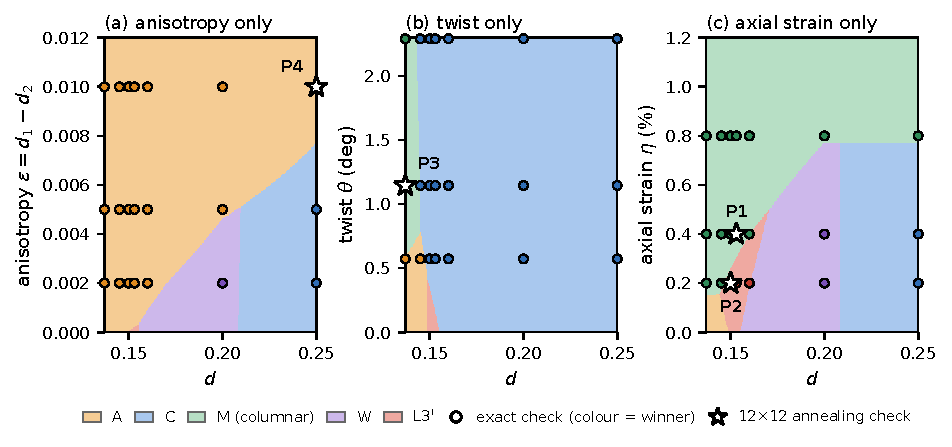
\includegraphics[width=\textwidth]{figs/fig5_deform.pdf}
\caption{Phase diagrams under (a) anisotropy, (b) twist and (c) axial strain for ideal islands, from zero-field energies and linear responses. Circles: exact energies at finite deformation (colour = winner); stars: $12\times12$ annealing checks. All checks agree with the estimate.}
\label{fig:deform}
\end{figure}

\section{Walls and island shape}

\subsection{Sharp, nearly free walls}

The wall crystals can be built line by line. W consists of lines of C and C$'$ cells separated by two kinds of wall lines; inserting $2k+1$ lines of each domain gives stripes with any wall spacing. L3$'$ can be generalised on the chessboard by stacking $m$ columnar layers between horizontal rows; spins follow from an inverse of the spin--dimer map, which is unique because each vertex status fixes a time-reversal pair of configurations. In both families the energy per wall cell is independent of the spacing to within 1--2\% (basketweave) and 6--10\% (columnar) [Fig.~\ref{fig:walls}(b)]. Walls are thus sharp lines that hardly interact, and whenever the wall tension is negative the densest wall crystal---W or L3$'$---wins.

\subsection{Wall tension from distant pairs: the moment ratio}

Decomposing $E_{\rm W}-E_{\rm C}$ into island pairs shows that all near pairs ($r<1.6a$) cancel identically: the wall tension is a delicate sum over distant pairs ($r\geq2.7a$). In this regime islands act as point dipoles, so island shape enters only through the moment ratio $\mu=m_{\rm long}/m_{\rm short}$ between partner and $z3$--$z4$ islands,
\begin{equation}
E_X-E_C=S_{SS}(d)+\mu\,S_{LS}(d)+\mu^2S_{LL}(d)\qquad\left[\text{units } \mu_0m_S^2/4\pi a^3\simeq300~\text{K}\right],
\label{eq:mu}
\end{equation}
where the three lattice sums depend only on geometry. For W, long--long pairs favour walls ($S_{LL}<0$) and long--short pairs oppose them ($S_{LS}>0$), so the wall tension changes sign at $\mu_c(d)=1.21$, $1.38$, $1.57$ and $1.77$ for $d=0.153$, $0.175$, $0.20$ and $0.25$ [Fig.~\ref{fig:walls}(a)]. For the columnar family all three coefficients are negative in the relevant range, so walls are always favourable and the uniform columnar crystal never wins at zero deformation: L3$'$ takes its place [Fig.~\ref{fig:walls}(c)]. Near $d_c$ the wall tension also tracks $E_A-E_C$ almost one to one: a C$|$C$'$ wall passes through the odd plateau, and becomes cheap when that plateau is nearly degenerate. Because the walls are one line wide, this dependence is linear rather than the square-root form of a continuum sine-Gordon wall.

The ideal model has $\mu=2$, close to $\mu_c$, which is why W and C were nearly degenerate there. Realistic islands with fixed vertex gaps have $\mu$ rising from $1.45$ at the equilateral Cairo point to $3.1$ at the Shakti point, well inside the W window. Realistic wall tensions agree with Eq.~\eqref{eq:mu} to within 5\% ($-130$ vs.\ $-125$~K per wall cell at $d=0.25$).

\begin{figure}[t]
\centering
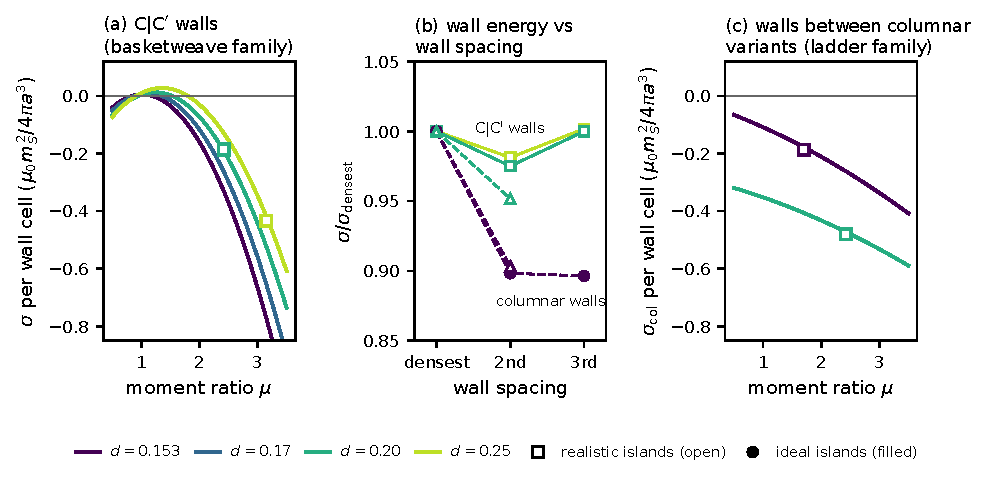
\includegraphics[width=\textwidth]{figs/fig6_walls.pdf}
\caption{Wall tensions. (a) C$|$C$'$ walls (basketweave family) from point-dipole lattice sums versus $\mu$; the zero crossing $\mu_c(d)$ is the W$|$C boundary. Open squares: realistic islands. (b) Energy per wall cell versus wall spacing, normalised to the densest arrangement: walls hardly interact. (c) Walls between columnar variants are favourable for all $\mu$, so L3$'$ replaces the uniform columnar crystal.}
\label{fig:walls}
\end{figure}

\subsection{The $(d,\mu)$ phase diagram}

Equation~\eqref{eq:mu} for all candidates yields the phase diagram of Fig.~\ref{fig:dmu}. W occupies the window $\mu_c(d)<\mu<\mu_A(d)$, with an upper boundary $\mu_A\simeq2.0$, $2.8$ and $3.3$ at $d=0.175$, $0.20$ and $0.25$ above which A wins (A gains as $\mu^2$, since $S_{LS}=0$ for A by symmetry). C survives only in a narrow band below $\mu_c$, and L3$'$ appears near $d_c$ at small $\mu$, where the $\mu^2$ advantage of A is weak while L3$'$ gains linearly. Realistic-island calculations at 35 points, with $\mu$ tuned through the partner-island length or width, agree with the analytic diagram at 33 of them; the two exceptions lie on the edge of the L3$'$ pocket, where competing states are within 1~K.

\begin{figure}[t]
\centering
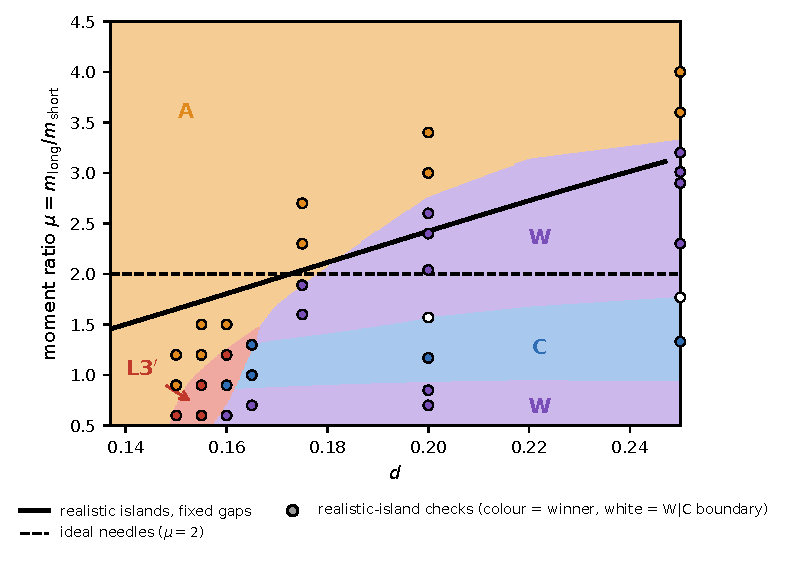
\includegraphics[width=0.66\textwidth]{figs/fig7_dmu.pdf}
\caption{Analytic phase diagram in the plane of geometry $d$ and moment ratio $\mu$, from Eq.~\eqref{eq:mu}. Solid line: realistic islands with fixed vertex gaps; dashed line: ideal needles. Circles: realistic-island calculations (colour = winner).}
\label{fig:dmu}
\end{figure}

\subsection{Thresholds for real islands}

The critical deformation that stabilises a crystal $X$ follows from
\begin{equation}
k^*_X=\frac{\Delta E_X}{\lambda_{k,X}},
\label{eq:threshold}
\end{equation}
where $\Delta E_X$ is the zero-field dipolar penalty of $X$ and $\lambda_{k,X}$ its vertex-level response. Island shape affects numerator and denominator differently. For anisotropy and twist both decrease together as vertex gaps open, and the thresholds grow by only 1.4--2.9 times; for axial strain the response of the columnar crystal is a near-field effect that collapses with the gaps, and the threshold grows by 7--8 times. Equation~\eqref{eq:threshold} reproduces direct calculations to within 10\%. For realistic islands [Fig.~\ref{fig:real}] the zero-field ground state is A up to $d\simeq0.175$ and W beyond, with C only 2--6~K per island above W. A twist of only $0.14$--$0.36^\circ$ turns W into C on the Shakti side, a displacement of the $z=3$ vertices by 1.5--6~nm turns it into A, and a twist of $0.7$--$1^\circ$ stabilises the columnar crystal on the Cairo side. Axial strain is a weak knob (3--7\%).

\begin{figure}[t]
\centering
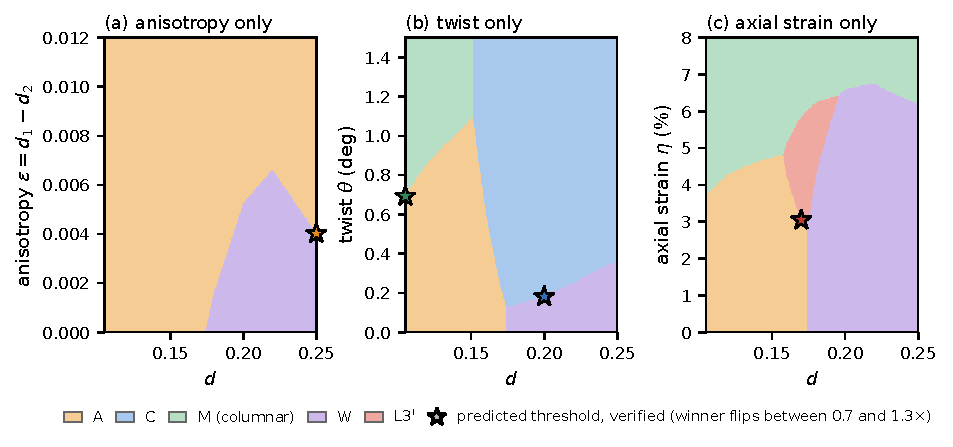
\includegraphics[width=\textwidth]{figs/fig8_real.pdf}
\caption{Phase diagrams for realistic islands under (a) anisotropy, (b) twist (degrees) and (c) axial strain (\%). Stars: thresholds from Eq.~\eqref{eq:threshold}, each verified by direct calculation (the winner changes between 0.7 and 1.3 times the predicted value).}
\label{fig:real}
\end{figure}

\section{Experiments and finite regions}

\subsection{Why annealed Cairo arrays are disordered}

The arrays of Ref.~\cite{Saccone2019} correspond to $d=0.105$, on the Cairo side. With their island geometry our couplings reproduce the micromagnetic couplings at the four-island vertices to within 15--35\%, and the ground state is A. The measured near-equal populations of the two types of three-island vertices are exactly the manifold prediction (one unhappy vertex per domino), and at the largest spacing $c=600$~nm, where we find that the happy--unhappy splitting collapses to about 20~K, the populations approach the degeneracy ratio 1:2, as observed (40:60). Manifold Monte Carlo gives an A ordering temperature $T_A=322$, $432$ and $562$~K for $c=376$, $450$ and $500$~nm. Inverting the measured four-island vertex populations with our vertex energies gives an effective freezing temperature of about 1300--2000~K, consistently from two independent population ratios [Fig.~\ref{fig:expt}]. The arrays therefore froze far above $T_A$, which explains the short-range correlations. The ratio $T_A/T_{\rm eff}$ grows with $c$, so arrays with $c\approx500$~nm are the closest to ordering. The vertex-level identity also implies that real fabrication anisotropy at the nanometre scale can decide which crystal forms.

\begin{figure}[t]
\centering
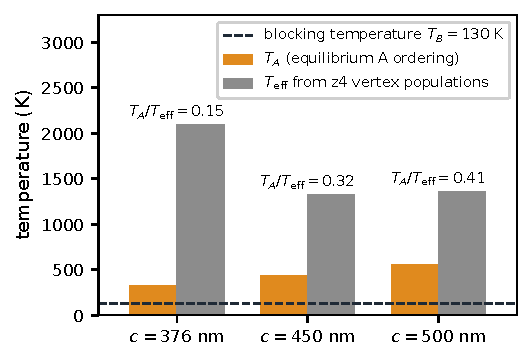
\includegraphics[width=0.52\textwidth]{figs/fig9_saccone.pdf}
\caption{Equilibrium A ordering temperature $T_A$ and effective freezing temperature $T_{\rm eff}$ inferred from the measured four-island vertex populations of Ref.~\cite{Saccone2019}.}
\label{fig:expt}
\end{figure}

\subsection{Boundaries select the plateau}

In finite samples the boundary fixes the height function and hence the plateau. We test this in Aztec-diamond regions with a minimal model that stabilises basketweave crystals and contains a bias $\delta$ between even and odd plateaus, so that the bulk A$|$C point is $\delta=0$. At $\delta=0$ the ground state alternates with the size parity [Fig.~\ref{fig:aztec}]: the central-plaquette (C) class for odd $n$ and the other (A) class for even $n$, with $\lfloor(n+1)^2/4\rfloor$ blocks in each case. The plateau height relative to the central vertex is $\pm(n+1)$ mod 4, so that the C variant is fixed by $n$ mod 4 while the two A variants are degenerate. The boundary shifts the A$|$C point by $|\delta^*(n)|\simeq1.4/n$, the ratio of perimeter to area. The same sign rule governs the sublattice contrast of local $2\times2$ correlations in uniformly random Aztec-diamond tilings~\cite{Won2026}, where the exact mean central height is $(-1)^{n+1}n$. For arrays of 30--40 cells the boundary shifts phase boundaries by a few per cent, enough to make the observed crystal depend on the sample size near a phase boundary, provided the edges are terminated so as to pin the height.

\begin{figure}[t]
\centering
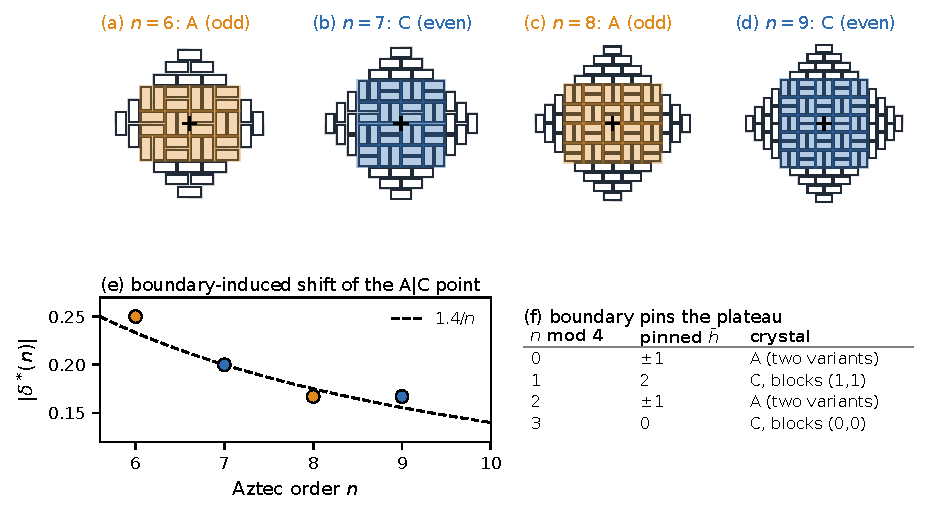
\includegraphics[width=\textwidth]{figs/fig10_aztec.pdf}
\caption{(a)--(d) Ground states of small Aztec diamonds at the bulk A$|$C point: the basketweave class alternates with the parity of $n$ (blue: even class containing the central plaquette; orange: odd class). (e) Boundary-induced shift of the transition point. (f) The pinned plateau height and the selected crystal.}
\label{fig:aztec}
\end{figure}

\section{Discussion and conclusion}

The Cairo--Shakti family shows how far a single topological fact---the dimer manifold---organises the physics of a frustrated magnet. Because the manifold is fixed by topology, everything else is selection, and selection is organised by the height field: integer plateaus (A, C), half-integer plateaus (columnar), and dense crystals of sharp walls (W, L3$'$). Each layer of the problem reduces to one controlling quantity. The sign of $\delta$ chooses between odd and even plateaus; the sign of a wall tension, set by distant islands through the moment ratio $\mu$, decides whether walls proliferate; symmetry decides which deformation couples to which crystal, and the exact vertex identity fixes the strength. None of these statements depends on the details of the island model: they rest on the topology of the manifold, on symmetry, and on the point-dipole limit for distant pairs, which is why the ideal and realistic models give the same structure with shifted boundaries.

Several predictions follow for experiments. (1) Any ice-rule-obeying region has exactly half closed pentagons, and equal numbers of the two three-island vertex types. (2) The Shakti-side ground state of realistic arrays is the wall crystal W rather than C, and it lies close to both C and A, so that small, deliberately designed twists or anisotropies should select C or A. (3) The moment ratio $\mu$ is a design parameter: shortening or narrowing the long islands to $\mu\approx1$--$1.7$ favours C, and $\mu\approx1$ near $d_c$ favours the ladder crystal. (4) Cairo arrays should approach A order when annealed slowly at spacings $c\approx500$~nm. (5) In finite, height-pinning geometries the selected crystal depends on the parity of the size.

Several questions remain. The finite-temperature A transition near $d_c$ requires larger multicanonical calculations to decide between weak first order and a crossover. The roughening picture implied by Eq.~\eqref{eq:F} remains qualitative. Finally, the same tools---dimer mapping, height plateaus and wall tensions---offer a route back to the pentagonal motifs of artificial quasicrystals, where the domain structures that motivated this work may be read as regions of forced plateaus separated by walls.

\section*{Acknowledgments}
The author thanks Kyung Hee University for support. The author used Claude (Anthropic) to assist with writing code for the numerical computations and figures and with editing the manuscript; all results were checked by the author, who takes full responsibility for the content.

\appendix
\section{Methods}
\label{app:methods}

\textbf{Couplings.} Ideal islands are needles divided into eight sub-dipoles per short edge (sixteen per long edge), with moment proportional to length. Pairs within $6a$ are evaluated with sub-dipoles and more distant pairs as point dipoles, summed over periodic images up to $64a$; phase labels are converged for cutoffs $\geq16a$. Realistic islands are stadia of $3\times\lceil\ell/19\,\text{nm}\rceil$ sub-dipoles with the subdivision fixed per island type from the undeformed lattice; pairs within $2.5a$ use sub-dipoles and the rest point dipoles up to $24a$. Energies are in kelvin with $M_s=790$~kA/m.

\textbf{Manifold and selection.} The manifold of the $4\times2$ cell was enumerated exhaustively and checked against dimer counts; zero-field energies of candidate crystals were compared on common tori ($12\times4$ for all candidates, $12\times12$ when all orientations are needed). Manifold Monte Carlo updates preserve the manifold by flipping $z=4$ vertices together with the partner islands they force; in deformed lattices the manifold constraint is checked with the undeformed vertex couplings.

\textbf{Linear responses and thresholds.} Responses are fixed-state derivatives with respect to $\varepsilon$, $\theta$ and $\eta$, with the best orientation of each crystal obtained from the symmetry $R:\varepsilon\to-\varepsilon$, $\eta\to-\eta$ and $M:\theta\to-\theta$. Thresholds follow from Eq.~\eqref{eq:threshold} including all competing candidates.

\textbf{Finite temperature.} Parallel tempering with multiple-histogram reweighting was used for the finite-size scaling at $d=0.145$ ($n=8$--24). Effective temperatures were obtained from Boltzmann ratios of the measured vertex populations.

\textbf{Aztec diamonds.} Ground states of $E=-\sum_pF_p(1+\delta s_p)+r\sum_{\langle pq\rangle}F_pF_q$ with $r=1$, where $F_p=1$ for a flippable plaquette and $s_p=(-1)^{x_p+y_p}$, were found by parallel tempering; mean heights of uniform tilings were computed from single-edge probabilities of the inverse Kasteleyn matrix.

\begin{thebibliography}{99}
\bibitem{Wang2006} R. F. Wang, C. Nisoli, R. S. Freitas, J. Li, W. McConville, B. J. Cooley, M. S. Lund, N. Samarth, C. Leighton, V. H. Crespi, and P. Schiffer, Nature (London) \textbf{439}, 303 (2006).
\bibitem{Nisoli2013} C. Nisoli, R. Moessner, and P. Schiffer, Rev. Mod. Phys. \textbf{85}, 1473 (2013).
\bibitem{Skjaervo2020} S. H. Skj{\ae}rv{\o}, C. H. Marrows, R. L. Stamps, and L. J. Heyderman, Nat. Rev. Phys. \textbf{2}, 13 (2020).
\bibitem{Moller2009} G. M{\"o}ller and R. Moessner, Phys. Rev. B \textbf{80}, 140409(R) (2009).
\bibitem{Morrison2013} M. J. Morrison, T. R. Nelson, and C. Nisoli, New J. Phys. \textbf{15}, 045009 (2013).
\bibitem{Chern2013} G.-W. Chern, M. J. Morrison, and C. Nisoli, Phys. Rev. Lett. \textbf{111}, 177201 (2013).
\bibitem{Gilbert2014} I. Gilbert, G.-W. Chern, S. Zhang, L. O'Brien, B. Fore, C. Nisoli, and P. Schiffer, Nat. Phys. \textbf{10}, 670 (2014).
\bibitem{Stopfel2018} H. Stopfel, E. {\"O}stman, I.-A. Chioar, D. Greving, U. B. Arnalds, T. P. A. Hase, A. Stein, B. Hj{\"o}rvarsson, and V. Kapaklis, Phys. Rev. B \textbf{98}, 014435 (2018).
\bibitem{Lao2018} Y. Lao, F. Caravelli, M. Sheikh, J. Sklenar, D. Gardeazabal, J. D. Watts, A. M. Albrecht, A. Scholl, K. Dahmen, C. Nisoli, and P. Schiffer, Nat. Phys. \textbf{14}, 723 (2018).
\bibitem{Saccone2019} M. Saccone, K. Hofhuis, Y.-L. Huang, S. Dhuey, Z. Chen, A. Scholl, R. V. Chopdekar, S. van Dijken, and A. Farhan, Phys. Rev. Materials \textbf{3}, 104402 (2019).
\bibitem{Makarova2021} K. Makarova, V. Strongin, I. Titovets, A. Syrov, I. Zinchenko \emph{et al.}, Phys. Rev. E \textbf{103}, 042129 (2021).
\bibitem{RodriguezGallo2023a} C. Rodr{\'i}guez-Gallo, A. Ortiz-Ambriz, C. Nisoli, and P. Tierno, Commun. Phys. \textbf{6}, 113 (2023).
\bibitem{RodriguezGallo2023b} C. Rodr{\'i}guez-Gallo, A. Ortiz-Ambriz, C. Nisoli, and P. Tierno, New J. Phys. \textbf{25}, 103007 (2023).
\bibitem{Farmer2016} B. Farmer, V. S. Bhat, A. Balk, E. Teipel, N. Smith, J. Unguris, D. J. Keavney, J. T. Hastings, and L. E. De Long, Phys. Rev. B \textbf{93}, 134428 (2016).
\bibitem{Shi2018} D. Shi, Z. Budrikis, A. Stein, S. A. Morley, P. D. Olmsted, G. Burnell, and C. H. Marrows, Nat. Phys. \textbf{14}, 309 (2018).
\bibitem{Kasteleyn1961} P. W. Kasteleyn, Physica \textbf{27}, 1209 (1961).
\bibitem{Thurston1990} W. P. Thurston, Am. Math. Mon. \textbf{97}, 757 (1990).
\bibitem{Henley2010} C. L. Henley, Annu. Rev. Condens. Matter Phys. \textbf{1}, 179 (2010).
\bibitem{Fradkin2004} E. Fradkin, D. A. Huse, R. Moessner, V. Oganesyan, and S. L. Sondhi, Phys. Rev. B \textbf{69}, 224415 (2004).
\bibitem{Alet2005} F. Alet, J. L. Jacobsen, G. Misguich, V. Pasquier, F. Mila, and M. Troyer, Phys. Rev. Lett. \textbf{94}, 235702 (2005).
\bibitem{Won2026} C. Won, \emph{Parity-dependent sublattice structure of local $2\times2$ correlations in domino tilings of the Aztec diamond} (in preparation).
\end{thebibliography}

\end{document}
